\documentclass{article}
\usepackage{amsmath, sfmath, multicol, tkz-euclide, array, enumerate, tcolorbox, tabularray, tipa}
\renewcommand{\familydefault}{\sfdefault}
\setlength{\parindent}{0cm}
\pagestyle{empty}
\usepackage[left=1in, top=0.5in, right=1in, bottom=0.5in]{geometry}
\tikzset{>=stealth, label style/.append style={font=\footnotesize}}
\tcbset{colback=white}

\newcounter{example}[section]
\newenvironment{example}[1][]{\refstepcounter{example}\par\medskip
   {\color{red}\textbf{Example~\theexample. #1}}}{\medskip}

\newcommand{\arc}[1]{%
    \setbox9=\hbox{#1}%
    \ooalign{\resizebox{\wd9}{\height}{\texttoptiebar{\phantom{A}}}\cr#1}}

\begin{document}

\section*{Experimental and Theoretical Probability}

\begin{tcolorbox}[colframe=orange!70!white, coltitle=black, title=\textbf{Today I Can}]
\begin{enumerate}
    \item Calculate experimental and theoretical probability.
\end{enumerate}
\end{tcolorbox}
\smallskip 

\begin{tcolorbox}[colframe=black!20!white, opacitybacktitle=0.1, coltitle=black, title=\textbf{Outcome}]
The possible result of a situation or experiment.
\end{tcolorbox}
\smallskip 

\begin{tcolorbox}[colframe=black!20!white, opacitybacktitle=0.1, coltitle=black, title=\textbf{Event}]
A single outcome or a group of outcomes.
\end{tcolorbox}
\smallskip 

\begin{tcolorbox}[colframe=black!20!white, opacitybacktitle=0.1, coltitle=black, title=\textbf{Sample Space}]
The set of all possible outcomes.
\end{tcolorbox}
\smallskip 

\begin{tcolorbox}[colframe=black!20!white, opacitybacktitle=0.1, coltitle=black, title=\textbf{Probability}]
The \textbf{probability} of an event, denoted $P$(event), is a numerical value from 0 to 1 that measures the likelihood of the event.

\begin{itemize}
    \item $P(\text{event}) = \dfrac{\text{number of favorable outcomes}}{\text{number of possible outcomes}}$
\end{itemize}
\end{tcolorbox}
\smallskip 

\begin{center}
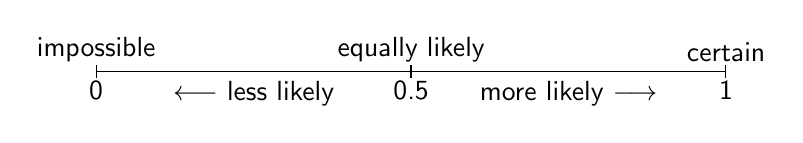
\begin{tikzpicture}
\draw [|-|] (0,0) -- (4,0);
\draw [|-|] (4,0) -- (8,0);
\node at (0,0) [above] {impossible};
\node at (0,0) [below] {0};
\node at (4,0) [above] {equally likely};
\node at (4,0) [below] {0.5};
\node at (8,0) [above] {certain};
\node at (8,0) [below] {1};
\node at (2,0) [below] {$\longleftarrow$ less likely};
\node at (6,0) [below] {more likely $\longrightarrow$};
\end{tikzpicture}
\end{center}
\bigskip 

\begin{tcolorbox}[colframe=black!20!white, opacitybacktitle=0.1, coltitle=black, title=\textbf{Experimental Probability}]
The measure of the likelihood that the event occurs based on the \emph{actual results} of an experiment.

\begin{itemize}
    \item $P(\text{event}) = \dfrac{\text{number of times the event occurs}}{\text{number of times the experiment is done}} = \dfrac{\text{number of favorable outcomes}}{\text{number of possible outcomes}}$
\end{itemize}
\end{tcolorbox}
\bigskip 

\begin{example}
A quality control inspector samples 500 LCD monitors and finds defects in three of them.

\begin{enumerate}[(a)]  \setlength{\itemsep}{0.75in}
    \item What is the experimental probability that a monitor selected at random will have a defect?
    \item If the company manufactures 15,240 monitors in a month, how many are likely to have a defect based on the quality inspector's results?
\end{enumerate}
\end{example}

\vfill 
\newpage 

\begin{tcolorbox}[colframe=black!20!white, opacitybacktitle=0.1, coltitle=black, title=\textbf{Theoretical Probability}]
The likelihood of an event based on mathematical reasoning.
\end{tcolorbox}
\bigskip 

\begin{example}
You roll two standard six-sided dice. The outcomes of which are shown in the table below.
\begin{center}
\begin{tabular}{c|c|c|c|c|c|c}
       \textbf{Dice} & \textbf{1} & \textbf{2} & \textbf{3} & \textbf{4} & \textbf{5} & \textbf{6} \\ \hline 
       \textbf{1} & 1,1 & 1,2 & 1,3 & 1,4 & 1,5 & 1,6 \\ \hline 
       \textbf{2} & 2,1 & 2,2 & 2,3 & 2,4 & 2,5 & 2,6 \\ \hline 
       \textbf{3} & 3,1 & 3,2 & 3,3 & 3,4 & 3,5 & 3,6 \\ \hline 
       \textbf{4} & 4,1 & 4,2 & 4,3 & 4,4 & 4,5 & 4,6 \\ \hline 
       \textbf{5} & 5,1 & 5,2 & 5,3 & 5,4 & 5,5 & 5,6 \\ \hline 
       \textbf{6} & 6,1 & 6,2 & 6,3 & 6,4 & 6,5 & 6,6
\end{tabular}
\end{center}
\bigskip 

What is the probability of getting each sum when rolling two standard dice?
\begin{multicols}{4}
    \begin{enumerate}[(a)]
        \item 7
        \item 9
        \item 2
        \item 13
    \end{enumerate}
\end{multicols}
\end{example}

\vfill 

\begin{tcolorbox}[colframe=black!20!white, opacitybacktitle=0.1, coltitle=black, title=\textbf{Complement of an Event}]
All possible outcomes of the sample space that are \textbf{not} part of the event.

\begin{itemize}
    \item The sum of the probability of an event and the probability of its complement is 1.
    \item $P(\text{event}) + P(\text{not event}) = 1$
    \item $P(\text{not event}) = 1 - P(\text{event})$
\end{itemize}
\end{tcolorbox}
\bigskip 

\begin{example}
A jar contains 10 red marbles, 8 green marbles, 5 blue marbles, and 6 white marbles. A marble is chosen at random. Find each probability. \bigskip 

\begin{multicols}{2}
\begin{enumerate}[(a)]
    \item Probability the marble is not green.
    \item Probability the marble is not red.
\end{enumerate}
\end{multicols}
\end{example}

\vfill 

\end{document}
